% ============================================================================
% CAPÍTULO 4 — EFS4AC
% Arquivo preparado para inclusão no projeto principal da dissertação.
%
% Observações:
% 1) O capítulo foi estruturado como um capítulo metodológico de dissertação,
%    apresentando a proposta, a arquitetura em etapas, as decisões de projeto
%    e a integração com a classificação associativa.
% 2) Mantém o label cap:Metodologia para não quebrar referências anteriores e
%    adiciona um label específico do método.
% 3) Pacotes recomendados no preâmbulo do projeto: amsmath, amssymb, array.
% ============================================================================
\chapter{\textit{EFS4AC}: Método de \textit{Ensemble Feature Selection} para Classificação Associativa}
\label{cap:Metodologia}

Este capítulo apresenta o método proposto nesta dissertação, denominado
\textit{EFS4AC}. A proposta foi concebida para incorporar \textit{Ensemble
Feature Selection} (EFS) ao contexto da classificação associativa, de modo a
selecionar um subconjunto de atributos antes da indução das regras de
classificação. A ideia central consiste em combinar diferentes métodos de
\textit{feature selection}, transformar suas saídas em \textit{rankings}
comparáveis, analisar a diversidade entre os \textit{rankings} produzidos, agregar
essas evidências em um consenso e, por fim, definir o subconjunto final
de atributos a ser utilizado pelo classificador associativo.

A motivação do \textit{EFS4AC} decorre de três constatações principais.
Primeiramente, a literatura mostra que diferentes métodos de FS capturam
critérios distintos de relevância, redundância e interação entre atributos,
de forma que a escolha de um único seletor pode introduzir dependência excessiva
de uma única perspectiva de avaliação \cite{bolon2019ensembles,salman2026review}.
Em segundo lugar, no contexto dos classificadores associativos, o número de atributos influencia diretamente o espaço de busca das regras, podendo afetar a complexidade do modelo final. Por fim,
a revisão realizada neste trabalho evidenciou que a aplicação de EFS à
classificação associativa ainda é pouco explorada, especialmente no que se
refere à investigação de diferentes estratégias de composição, diversidade,
agregação e seleção do subconjunto final de atributos.

Diferentemente de abordagens que alteram diretamente o mecanismo interno do
classificador associativo, o \textit{EFS4AC} atua como uma etapa anterior à
indução do modelo. Assim, o método não modifica a estrutura básica do
classificador associativo adotado; em vez disso, ele controla quais atributos
serão disponibilizados à mineração das regras. Essa decisão metodológica
favorece a modularidade da proposta e permite sua avaliação em diferentes
configurações de classificação associativa, bem como sua comparação com
abordagens sem seleção de atributos e com métodos individuais de FS.

A arquitetura do \textit{EFS4AC} contempla diferentes alternativas metodológicas para a composição dos métodos-base, o controle da diversidade, a agregação dos \textit{rankings} e a definição do subconjunto final de atributos. Essas alternativas constituem possibilidades de investigação que poderão ser implementadas, avaliadas e refinadas progressivamente ao longo da pesquisa. Os experimentos iniciais apresentados nesta dissertação, até a etapa de qualificação, não necessariamente contemplam todas as configurações propostas, podendo seus resultados orientar as decisões metodológicas e os experimentos posteriores.

%============================================================================
\section{Descrição do Método}\label{sec:ac-efs-visao-geral}
%============================================================================

A estrutura do \textit{EFS4AC} foi definida com base nas principais decisões metodológicas identificadas nos estudos de \textit{Ensemble Feature Selection} analisados no Capítulo~\ref{trabRelac}. Esses estudos evidenciam diferentes estratégias para a composição dos seletores, a representação de suas saídas, o tratamento da diversidade, a agregação dos resultados e a definição do subconjunto final de atributos. Considerando essas dimensões, o \textit{EFS4AC} organiza tais decisões em cinco etapas, priorizando estratégias baseadas em \textit{rankings} e sua aplicação à classificação associativa.

A escolha pela agregação de \textit{rankings} busca favorecer a flexibilidade do \textit{EFS4AC}, permitindo integrar métodos de \textit{feature selection} heterogêneos que produzem ordenações ou pontuações de relevância dos atributos. Essa representação estabelece uma base comum para a agregação, sem exigir a comparação direta de \textit{scores} com diferentes escalas e interpretações. Além disso, evita a necessidade de definir previamente um subconjunto de atributos para cada método-base, reduzindo decisões adicionais de parametrização. Assim, o \textit{EFS4AC} foi concebido como um \textit{pipeline} flexível, que busca limitar a introdução de hiperparâmetros sempre que possível, concentrando a definição do subconjunto final de atributos após a agregação dos \textit{rankings}.

O \textit{EFS4AC} é estruturado em cinco etapas, conforme apresentado
na Figura~\ref{fig:fluxo-geral-ac-efs}. Inicialmente, são selecionados
os métodos-base de \textit{feature selection} que irão compor o
\textit{ensemble}. Em seguida, esses métodos são aplicados aos dados para
produzir \textit{rankings} individuais dos atributos, os quais são padronizados
para permitir sua comparação. Na terceira etapa, a diversidade entre
os \textit{rankings} é analisada, podendo ser utilizadas estratégias para
controlar a redundância entre os seletores. Posteriormente, os \textit{rankings}
são agregados para produzir um \textit{ranking} consensual, a partir do qual
é definido o subconjunto final de atributos.

%%%%%%%%%
\begin{figure}[htbp]
    \centering
    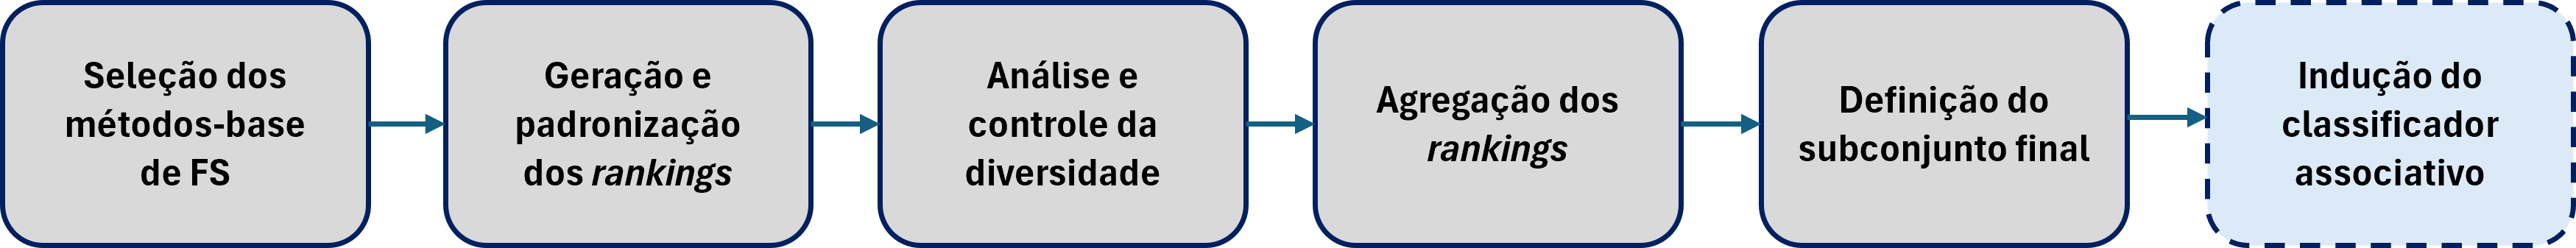
\includegraphics[width=\textwidth]{figuras/EFS4AC.png}
    \caption{Fluxo geral do método \textit{EFS4AC} e sua integração
    com a classificação associativa.}
    \label{fig:fluxo-geral-ac-efs}
\end{figure}
%%%%%%%%%

O subconjunto de atributos resultante constitui a saída do
\textit{EFS4AC} e é utilizado na indução do classificador associativo.
Dessa forma, a seleção de atributos é realizada previamente à
construção do modelo, sem modificar os procedimentos internos de
mineração, ordenação e poda das regras. As etapas do método são
detalhadas nas seções seguintes.

%===========================================================================
\subsection{Seleção dos Métodos-Base de FS}\label{sec:ac-efs-etapa1}
%============================================================================

A primeira etapa do \textit{EFS4AC} consiste na definição dos métodos-base de \textit{feature selection} que irão compor o \textit{ensemble}. Essa escolha determina as diferentes perspectivas de avaliação da relevância dos atributos que serão consideradas na construção do consenso. Neste trabalho, optou-se pela utilização de métodos supervisionados da categoria \textit{filter}, que não dependem diretamente do classificador utilizado posteriormente e permitem combinar diferentes critérios estatísticos e informacionais. A seleção dos métodos-base considera quatro critérios principais:
\begin{itemize}
    \item \textbf{Compatibilidade com dados discretizados}: os métodos devem ser aplicáveis à representação dos atributos utilizada na classificação associativa;

    \item \textbf{Aplicabilidade a problemas com classe nominal}: os métodos devem operar em problemas de classificação, incluindo cenários binários e multiclasse;

    \item \textbf{Capacidade de produzir \textit{rankings} completos}: os métodos devem permitir, diretamente ou a partir de suas pontuações, estabelecer uma ordenação de todos os atributos avaliados;

    \item \textbf{Diversidade dos critérios de avaliação}: busca-se combinar métodos que considerem diferentes aspectos da relevância dos atributos, incluindo associação estatística, dependência informacional, redundância e interação entre atributos.
\end{itemize}

Os três primeiros critérios estabelecem requisitos de compatibilidade com a arquitetura do \textit{EFS4AC}, enquanto o último orienta a composição de um \textit{ensemble} heterogêneo. Cabe destacar que a diversidade considerada nesta etapa é conceitual, decorrente dos diferentes critérios empregados pelos métodos. A diversidade efetivamente observada entre os \textit{rankings} será analisada posteriormente.

Após a análise de diferentes bibliotecas de seleção de atributos, adotou-se a biblioteca \textit{ITMO-FS}\footnote{\url{https://itmo-fs.readthedocs.io/en/latest/index.html}.} como referência para a implementação dos métodos-base. Entre os métodos disponíveis nessa biblioteca, foram selecionados inicialmente dez, apresentados na Tabela~\ref{tab:metodos-base-ac-efs}. Eles compreendem quatro métodos univariados, que avaliam a relevância dos atributos individualmente em relação à classe, e seis métodos multivariados ou sequenciais, que também consideram relações entre atributos durante o processo de seleção.

%%%%%%%%%%%%%%
%%%%%%%%%%%%%%
\begin{table}[ht]
    \centering
    \small
    \caption{Métodos-base da configuração inicial do \textit{EFS4AC}.}
    \label{tab:metodos-base-ac-efs}

    \begin{tabular}{p{2.0cm} p{3.0cm} p{7.2cm}}
        \hline
        \textbf{Método} &
        \textbf{Tipo} &
        \textbf{Critério predominante} \\
        \hline

        Gini
        & Univariado
        & Discriminação das classes a partir da distribuição dos dados. \\

        $\chi^2$
        & Univariado
        & Associação estatística entre o atributo e a classe. \\

        SU
        & Univariado
        & Dependência informacional normalizada entre atributo e classe. \\

        MIM
        & Univariado
        & Relevância individual baseada em informação mútua com a classe. \\

        \hline

        MRMR
        & Multivariado
        & Maximização da relevância e redução da redundância. \\

        JMI
        & Multivariado
        & Relevância conjunta e informação complementar entre atributos. \\

        CIFE
        & Multivariado
        & Relevância condicionada e interação com atributos selecionados. \\

        CMIM
        & Multivariado
        & Informação mútua condicional em relação aos atributos selecionados. \\

        ICAP
        & Multivariado
        & Relevância, redundância e efeitos de interação entre atributos. \\

        MRI
        & Multivariado
        & Relevância considerando redundância e interação informacional. \\

        \hline
    \end{tabular}
\end{table}
%%%%%%%%%%%%%%
%%%%%%%%%%%%%%

Além desses métodos, foram considerados também MIFS, DCSF, CFR, IWFS e DISR. Entretanto, sua inclusão foi reservada para investigações posteriores, devido à necessidade de parametrizações adicionais ou de adaptações específicas para a geração de \textit{rankings} completos. Essa decisão busca preservar a flexibilidade do \textit{EFS4AC}, evitando aumentar desnecessariamente a complexidade de configuração do método.

A arquitetura proposta permite diferentes composições do \textit{ensemble}. Neste trabalho, são consideradas três possibilidades: uma composição formada apenas por métodos univariados ($E_U$), outra formada apenas por métodos multivariados ou sequenciais ($E_M$) e uma composição que reúne ambos os grupos ($E_{U+M}$). A composição $E_{U+M}$ é considerada inicialmente como configuração principal do \textit{EFS4AC}, por reunir métodos com diferentes critérios de avaliação, enquanto as demais permitem investigar o comportamento do método com diferentes conjuntos de seletores. A escolha da configuração final poderá ser revista a partir dos resultados experimentais.

A saída desta etapa é o conjunto de métodos-base que será utilizado na geração dos \textit{rankings} individuais dos atributos.

%===========================================================================
\subsection{Geração e Padronização dos \textit{Rankings}}\label{sec:ac-efs-etapa2}
%============================================================================

A segunda etapa do \textit{EFS4AC} consiste na aplicação dos métodos-base selecionados na etapa anterior e na conversão de suas saídas em uma representação comum, baseada em \textit{rankings} completos dos atributos. Essa padronização permite combinar métodos que utilizam diferentes critérios de avaliação, sem exigir a comparação direta de \textit{scores} com escalas e interpretações distintas.

A obtenção dos \textit{rankings} depende do funcionamento dos métodos-base. Nos métodos univariados, como Gini, $\chi^2$, SU e MIM, os atributos são ordenados de acordo com seus \textit{scores} individuais de relevância. Já nos métodos multivariados ou sequenciais, como MRMR, JMI, CIFE, CMIM, ICAP e MRI, o \textit{ranking} é determinado pela ordem de seleção dos atributos, considerando as relações com aqueles previamente selecionados. Em ambos os casos, o procedimento deve produzir uma ordenação completa dos atributos.

Seja $F=\{f_1,f_2,\ldots,f_n\}$ o conjunto de atributos e $S_j$ um dos $M$ métodos-base. O \textit{ranking} produzido pelo seletor $S_j$ é representado via Equação~\ref{eq:ranking-individual-ac-efs}, em que $r_j(f_i)$ corresponde à posição atribuída ao atributo $f_i$ pelo método $S_j$. Todos os \textit{rankings} seguem a mesma convenção: a posição 1 corresponde ao atributo considerado mais relevante, enquanto a posição $n$ corresponde ao menos relevante. Quando necessário, o sentido de preferência dos \textit{scores} é ajustado antes da ordenação. Eventuais empates entre os \textit{scores} são tratados pelo método dos postos médios (\textit{average ranks}), no qual atributos empatados recebem a média das posições que ocupariam na ordenação. Dessa forma, todos os atributos recebem uma posição, preservando-se os empates sem introduzir critérios arbitrários de desempate.

%%%%%%%%%%
\begin{equation}\label{eq:ranking-individual-ac-efs}
    R_j =
    \left(
        r_j(f_1),
        r_j(f_2),
        \ldots,
        r_j(f_n)
    \right)
\end{equation}
%%%%%%%%%%

Após a execução dos $M$ métodos-base, os \textit{rankings} são organizados em uma matriz de posições $\mathbf{R}\in\mathbb{R}^{n\times M}$, conforme Equação~\ref{eq:matriz-ranks-ac-efs}. Nessa matriz, cada linha representa um atributo e cada coluna corresponde ao \textit{ranking} produzido por um método-base. A matriz $\mathbf{R}$ constitui a saída desta etapa e será utilizada na análise da diversidade e na agregação dos \textit{rankings}.

%%%%%%%%%%
\begin{equation}\label{eq:matriz-ranks-ac-efs}
    \mathbf{R}=
    \begin{bmatrix}
        r_1(f_1) & r_2(f_1) & \cdots & r_M(f_1) \\
        r_1(f_2) & r_2(f_2) & \cdots & r_M(f_2) \\
        \vdots   & \vdots   & \ddots & \vdots   \\
        r_1(f_n) & r_2(f_n) & \cdots & r_M(f_n)
    \end{bmatrix}
\end{equation}
%%%%%%%%%%

%===========================================================================
\subsection{Análise e Controle da Diversidade dos \textit{Rankings}}\label{sec:ac-efs-etapa3}
%============================================================================

A terceira etapa do \textit{EFS4AC} consiste na análise da similaridade entre os \textit{rankings} produzidos pelos métodos-base, buscando identificar e controlar possíveis redundâncias antes da agregação. Embora os métodos tenham sido selecionados por utilizarem diferentes critérios de avaliação, essa diversidade conceitual não garante que produzam \textit{rankings} empiricamente distintos. Assim, seletores com ordenações muito semelhantes podem aumentar a influência de uma mesma preferência sobre o resultado agregado.

A concordância entre os \textit{rankings} é avaliada por meio do coeficiente de correlação de postos de Spearman. A escolha de Spearman deve-se à sua adequação à comparação de ordenações completas, permitindo avaliar a concordância global entre as posições atribuídas aos atributos. Embora outras medidas, como Kendall, também sejam aplicáveis, optou-se por fixar Spearman como medida de referência, concentrando a investigação experimental nas estratégias de controle da redundância. Assim, para dois \textit{rankings} $R_i$ e $R_j$, sua similaridade é representada via Equação~\ref{eq:spearman-ac-efs}. Valores próximos de 1 indicam elevada concordância entre as ordenações, enquanto valores próximos de zero indicam baixa associação monotônica e valores próximos de $-1$ representam ordenações aproximadamente inversas. As correlações calculadas entre todos os pares de métodos-base são organizadas em uma matriz de similaridade $\mathbf{S}$.

\begin{equation}\label{eq:spearman-ac-efs}
    \rho_{ij}=\rho(R_i,R_j),
    \qquad -1\leq\rho_{ij}\leq1
\end{equation}

A partir dessa matriz, o \textit{EFS4AC} contempla três configurações para investigar o efeito do controle da redundância entre os \textit{rankings}:
\begin{enumerate}
    \item \textbf{Sem controle de redundância ($D_0$):} todos os \textit{rankings} produzidos na etapa anterior são preservados para a agregação. Essa configuração constitui o cenário de referência, permitindo avaliar se a aplicação de mecanismos de controle proporciona benefícios ao \textit{EFS4AC}.

    \item \textbf{Controle por limiar de similaridade ($D_L$):} \textit{rankings} cuja correlação de Spearman seja superior ou igual a um limiar $\tau$ são considerados potencialmente redundantes. O controle é realizado de forma iterativa, identificando-se o par de \textit{rankings} com maior similaridade e removendo-se um de seus integrantes. Para a remoção, prioriza-se o \textit{ranking} com maior similaridade média em relação aos demais, por representar uma preferência potencialmente mais redundante. O procedimento é repetido até que nenhum par restante apresente correlação superior ou igual ao limiar estabelecido.

    \item \textbf{Controle por agrupamento ($D_C$):} utiliza-se agrupamento hierárquico para identificar conjuntos de \textit{rankings} semelhantes. A escolha do agrupamento hierárquico deve-se à possibilidade de identificar diferentes níveis de similaridade entre os \textit{rankings}, sem exigir a definição prévia do número de grupos. Essa característica permite investigar diferentes critérios de corte e observar como a composição dos grupos influencia a seleção dos representantes. Para isso, a matriz de similaridade é convertida em uma matriz de dissimilaridade, definida por $d_{ij}=1-\rho_{ij}$. Os grupos são definidos a partir de um critério de corte, e um representante de cada grupo é selecionado para participar da agregação. Como critério de representatividade, utiliza-se a menor dissimilaridade média em relação aos demais integrantes do grupo, preservando o \textit{ranking} mais central de cada agrupamento.
\end{enumerate}

As estratégias $D_L$ e $D_C$ buscam reduzir a influência de \textit{rankings} semelhantes por meio da seleção de representantes, diferenciando-se pela forma de identificar a redundância. Enquanto $D_L$ utiliza diretamente as similaridades entre pares de \textit{rankings}, $D_C$ considera a estrutura de agrupamento do conjunto de seletores.

Os valores de limiar, os procedimentos de agrupamento e os critérios de corte constituem aspectos a serem definidos e investigados ao longo da pesquisa. A avaliação experimental poderá contemplar progressivamente essas configurações, buscando verificar se o controle explícito da redundância contribui para o desempenho do \textit{EFS4AC}, sem pressupor que uma maior diversidade entre \textit{rankings} resulte necessariamente em melhores classificadores.

A saída desta etapa corresponde ao conjunto de \textit{rankings} preservados pela estratégia adotada, que será utilizado na etapa seguinte para a construção do \textit{ranking} consensual. A matriz de similaridade também constitui uma saída analítica, permitindo caracterizar a concordância entre os diferentes métodos-base. A arquitetura do \textit{EFS4AC} também permite investigar outras estratégias de controle da redundância, como a ponderação dos \textit{rankings} com base em sua similaridade, em vez da seleção de representantes. Essas alternativas poderão ser exploradas em etapas futuras da pesquisa.

%===========================================================================
\subsection{Agregação dos \textit{Rankings}}
\label{sec:ac-efs-etapa4}
%===========================================================================

A quarta etapa do \textit{EFS4AC} consiste na combinação dos \textit{rankings} provenientes da etapa anterior, com o objetivo de produzir uma ordenação consensual dos atributos. Enquanto a Etapa 3 permite analisar e, quando aplicável, controlar a redundância entre os seletores, esta etapa busca integrar suas diferentes perspectivas de relevância em uma única ordenação.

Seja $\mathcal{R}^{*}=\{R_1^{*},R_2^{*},\ldots,R_{M'}^{*}\}$ o conjunto de \textit{rankings} disponibilizado pela Etapa 3, em que $M'$ representa o número de \textit{rankings} considerados na agregação. Para cada atributo $f_i$, um operador de agregação $\mathcal{A}$ combina as posições atribuídas pelos diferentes seletores, produzindo um \textit{score} consensual, a saber: $c(f_i)=\mathcal{A}\left(r_1^{*}(f_i),r_2^{*}(f_i),\ldots,r_{M'}^{*}(f_i)\right)$. A partir desses \textit{scores}, os atributos são ordenados para produzir o \textit{ranking} consensual. Dependendo do operador considerado, as posições dos atributos podem ser previamente transformadas em pontuações de preferência, conforme detalhado a seguir.

Como alternativas iniciais de agregação, o \textit{EFS4AC} considera variantes do método Borda, pertencente à área de agregação de \textit{rankings} \cite{ijcai2024p915}, e o \textit{Technique for Order Preference by Similarity to Ideal Solution} (TOPSIS), pertencente à área de análise de decisão multicritério \cite{WATROBSKI2019107}. A escolha desses mecanismos busca contemplar diferentes perspectivas de construção do consenso: enquanto Borda combina diretamente as preferências atribuídas pelos seletores, TOPSIS considera a proximidade dos atributos em relação a soluções ideais. Dessa forma, pretende-se investigar se diferentes mecanismos de agregação influenciam a seleção dos atributos e, consequentemente, o desempenho da classificação associativa.

\begin{enumerate}
    \item \textbf{Borda.} Combina as preferências dos seletores a partir das posições atribuídas aos atributos. Neste trabalho, são consideradas quatro variantes \cite{10.1093/bib/bbx101}: Borda Média (BM), Borda Mediana (BD), Borda Geométrica (BG) e Borda L2 (BL). Como as posições seguem a convenção de que valores menores representam maior relevância, elas são inicialmente convertidas em pontuações de preferência, a saber: $b_{ij}=n-r_j^{*}(f_i)+1$, em que $n$ corresponde ao número de atributos. Assim, valores maiores de $b_{ij}$ indicam maior preferência pelo atributo $f_i$.

    As quatro variantes diferenciam-se pela forma de combinar essas pontuações, a saber:

    \begin{itemize}
        \item \textbf{Borda Média (BM):} utiliza a média aritmética das pontuações atribuídas ao atributo pelos diferentes seletores (Equação~\ref{eq:borda-media-ac-efs});

        \begin{equation}\label{eq:borda-media-ac-efs}
            c_{\mathrm{BM}}(f_i)
            =
            \frac{1}{M'}
            \sum_{j=1}^{M'} b_{ij}
        \end{equation}

        \item \textbf{Borda Mediana (BD):} utiliza a mediana das pontuações, reduzindo a influência de avaliações extremas (Equação~\ref{eq:borda-mediana-ac-efs});

        \begin{equation}\label{eq:borda-mediana-ac-efs}
            c_{\mathrm{BD}}(f_i)
            =
            \operatorname{mediana}
            \left(b_{i1},b_{i2},\ldots,b_{iM'}\right)
        \end{equation}

        \item \textbf{Borda Geométrica (BG):} utiliza a média geométrica das pontuações (Equação~\ref{eq:borda-geometrica-ac-efs}):

        \begin{equation}\label{eq:borda-geometrica-ac-efs}
            c_{\mathrm{BG}}(f_i)
            =
            \left(
                \prod_{j=1}^{M'} b_{ij}
            \right)^{1/M'}
        \end{equation}

        \item \textbf{Borda L2 (BL):} combina as pontuações por meio de uma medida baseada na norma Euclidiana (Equação~\ref{eq:borda-l2-ac-efs}).

        \begin{equation}\label{eq:borda-l2-ac-efs}
            c_{\mathrm{BL}}(f_i)
            =
            \sqrt{
                \frac{1}{M'}
                \sum_{j=1}^{M'} b_{ij}^{2}
            }
        \end{equation}
    \end{itemize}

    A utilização dessas variantes permite investigar diferentes formas de combinar as preferências dos seletores. A média aritmética considera a contribuição de todas as pontuações de maneira linear, enquanto a mediana reduz a influência de avaliações extremas. A média geométrica é mais sensível a pontuações baixas, favorecendo atributos com avaliações mais equilibradas entre os seletores. Por sua vez, a variante L2 atribui maior influência às pontuações elevadas. Essas diferenças permitem examinar como o mecanismo de combinação das preferências afeta o consenso produzido. Em todas as variantes, valores maiores de $c(f_i)$ indicam maior preferência coletiva pelo atributo. As diferentes formas de agregação permitem investigar como o tratamento das posições atribuídas pelos seletores influencia a construção do \textit{ranking} consensual.

    \item \textbf{TOPSIS.} Considera a agregação como um problema de decisão multicritério, no qual os atributos representam as alternativas e os \textit{rankers} constituem os critérios de avaliação.

    As posições dos atributos são inicialmente convertidas em pontuações de preferência, utilizando a transformação definida anteriormente ($b_{ij}=n-r_j^{*}(f_i)+1$). Essas pontuações compõem uma matriz de decisão, cujas colunas são normalizadas. Considera-se inicialmente que todos os seletores possuem a mesma importância, sendo utilizados pesos uniformes.

    A partir da matriz normalizada e ponderada, são determinadas as soluções ideais positiva e negativa, correspondentes, respectivamente, aos melhores e piores valores observados em cada critério. Para cada atributo, calculam-se as distâncias $D_i^{+}$ e $D_i^{-}$ em relação a essas soluções. O \textit{score} consensual é obtido pelo coeficiente de proximidade à solução ideal, definido via Equação~\ref{eq:topsis-score-ac-efs}. Quanto maior esse coeficiente, maior a preferência pelo atributo. Diferentemente das variantes de Borda, o TOPSIS considera a proximidade relativa de cada atributo às soluções ideais para estabelecer a ordenação consensual.

    \begin{equation}\label{eq:topsis-score-ac-efs}
        c_{\mathrm{TOPSIS}}(f_i)
        =
        \frac{D_i^{-}}{D_i^{+}+D_i^{-}}
    \end{equation}
\end{enumerate}

As alternativas consideradas permitem investigar diferentes mecanismos de construção do consenso. Enquanto as variantes de Borda combinam diretamente as pontuações derivadas das posições, o TOPSIS avalia os atributos a partir de sua proximidade às soluções ideais. A comparação entre essas alternativas poderá ser realizada progressivamente ao longo da pesquisa, buscando identificar seus efeitos sobre a seleção de atributos e o desempenho da classificação associativa.

Independentemente do agregador utilizado, a saída desta etapa consiste em um \textit{score} consensual para cada atributo e no correspondente \textit{ranking} global $R^{*}$. A definição dos atributos que serão efetivamente mantidos ocorre na Etapa 5, preservando a separação entre a agregação dos \textit{rankings} e a determinação do subconjunto final de atributos.

A arquitetura do \textit{EFS4AC} também permite investigar outras alternativas de agregação, como o \textit{Reciprocal Rank Fusion} (RRF) \cite{Cormack2009RRF}, bem como estratégias de ponderação dos seletores. Essas possibilidades poderão ser exploradas em etapas futuras da pesquisa.

%===========================================================================
\subsection{Definição do Subconjunto Final de Atributos}\label{sec:ac-efs-etapa5}
%===========================================================================

A quinta etapa do \textit{EFS4AC} consiste na definição do subconjunto final de atributos a partir do \textit{ranking} consensual produzido na Etapa 4. Embora a agregação estabeleça uma ordenação global de preferência, é necessário determinar quantos atributos serão preservados para a indução do classificador associativo.

Seja $R^{*}=(f_{(1)},f_{(2)},\ldots,f_{(n)})$ o \textit{ranking} consensual, em que $f_{(1)}$ representa o atributo mais bem posicionado, e $c_{(i)}$ o \textit{score} de consenso associado ao atributo na posição $i$. O subconjunto final $F^{*}\subseteq F$ é formado pelos atributos que ocupam as primeiras $k^{*}$ posições do \textit{ranking}, sendo $k^{*}$ determinado por uma estratégia de corte.

Inicialmente, o \textit{EFS4AC} considera duas estratégias para definir esse ponto de corte: percentuais fixos e corte adaptativo baseado nos \textit{scores} de consenso.

\begin{enumerate}
    \item \textbf{Cortes percentuais fixos.} Consistem na seleção de uma proporção predefinida dos atributos mais bem posicionados no \textit{ranking} consensual. Seja $p\in(0,1]$ a proporção de atributos a ser preservada. O número de atributos selecionados é definido por $k_p=\left\lceil p\,n\right\rceil$. Inicialmente, serão considerados os percentuais de 25\%, 50\% e 75\%, permitindo avaliar o comportamento do método sob diferentes níveis de redução dimensional. Esses valores não pressupõem a existência de um percentual universalmente adequado, mas fornecem condições experimentais padronizadas para comparar os resultados.

    \item \textbf{Corte adaptativo baseado no consenso.} Busca determinar o ponto de corte a partir da distribuição dos \textit{scores} produzidos pela agregação, sem depender de percentuais predefinidos. Para representar os \textit{scores} produzidos pelos diferentes agregadores em uma escala comum, os valores são inicialmente normalizados para o intervalo $[0,1]$, conforme a Equação~\ref{eq:normalizacao-consenso-ac-efs}, em que $\ell=1,\ldots,n$ representa o índice dos atributos considerados na determinação dos valores mínimo e máximo.
    \begin{equation}\label{eq:normalizacao-consenso-ac-efs}
        \tilde{c}_{(i)}
        =
        \frac{
            c_{(i)}-\min_{\ell}c_{(\ell)}
        }{
            \max_{\ell}c_{(\ell)}
            -
            \min_{\ell}c_{(\ell)}
        }
    \end{equation}

    Caso todos os atributos apresentem o mesmo \textit{score} consensual, a normalização não poderá ser realizada e não haverá uma diferença que fundamente o corte adaptativo. Nessa situação, todos os atributos serão preservados.
    
    Considerando os atributos ordenados por preferência, a diferença entre os \textit{scores} normalizados de duas posições consecutivas é definida por $\Delta_i=\tilde{c}_{(i)}-\tilde{c}_{(i+1)}$, para $i=1,\ldots,n-1$. O ponto de corte é determinado pela maior diferença entre posições consecutivas, conforme a Equação~\ref{eq:corte-maior-queda-ac-efs}. Caso a maior diferença ocorra em mais de uma posição, será considerada sua primeira ocorrência, priorizando o menor subconjunto de atributos.

    \begin{equation}
        k_{\Delta}
        =
        \underset{1\leq i<n}{\arg\max}
        \left(
            \tilde{c}_{(i)}-\tilde{c}_{(i+1)}
        \right)
        \label{eq:corte-maior-queda-ac-efs}
    \end{equation}
    
    Essa estratégia interpreta uma queda acentuada no consenso como uma possível separação entre atributos mais e menos relevantes. A escolha desse critério deve-se à sua simplicidade e à possibilidade de determinar o subconjunto diretamente a partir dos resultados da agregação, sem exigir parâmetros adicionais ou a definição prévia do número de atributos. Entretanto, sua efetividade será avaliada experimentalmente, uma vez que a maior diferença entre os \textit{scores} não corresponde necessariamente ao ponto de corte mais adequado para a classificação.
\end{enumerate}

Independentemente da estratégia utilizada, o subconjunto final é formado pelos $k^{*}$ atributos mais bem posicionados no \textit{ranking} consensual, isto é, $F^{*}=\{f_{(1)},f_{(2)},\ldots,f_{(k^{*})}\}$. A proporção de redução obtida é calculada por $1-|F^{*}|/n$.

O conjunto de dados de treinamento é então reduzido aos atributos de $F^{*}$, e essa representação é utilizada na indução do classificador associativo. Dessa forma, a Etapa 5 encerra o processo de seleção de atributos do \textit{EFS4AC}, permitindo investigar os efeitos das diferentes estratégias de corte sobre a redução dimensional e o desempenho preditivo.

%============================================================================
\section{Considerações Finais}\label{sec:ac-efs-consideracoes}
%============================================================================

Este capítulo apresentou o \textit{EFS4AC}, um método de
\textit{Ensemble Feature Selection} baseado na agregação de
\textit{rankings}, proposto para atuar previamente à indução de
classificadores associativos. O método busca combinar diferentes
perspectivas de relevância dos atributos para produzir uma ordenação
consensual e definir um subconjunto a ser utilizado na classificação.

Uma característica da proposta é a separação entre as decisões
envolvidas no processo de seleção. A composição do \textit{ensemble},
a representação dos resultados dos seletores, o controle da
redundância, a construção do consenso e a definição do subconjunto
final são tratados como problemas distintos. Essa organização
confere modularidade ao \textit{EFS4AC}, permitindo investigar
diferentes configurações sem modificar sua estrutura geral.

As decisões metodológicas apresentadas ao longo do capítulo são
fundamentadas em estratégias identificadas nos trabalhos relacionados,
discutidos no Capítulo~\ref{trabRelac}. A Tabela~\ref{tab:fundamentacao-efs4ac}
sintetiza essa relação, destacando as estratégias utilizadas na
literatura e as decisões adotadas ou adaptadas no \textit{EFS4AC}.
As referências apresentadas são representativas, priorizando os
trabalhos mais diretamente relacionados à proposta, sem constituir
uma enumeração exaustiva dos estudos que empregam cada estratégia.

%%%%%%%%%%%%%%%%%%%%%%%
%%%%%%%%%%%%%%%%%%%%%%%
\begingroup
\footnotesize
\setlength{\tabcolsep}{3pt}
\renewcommand{\arraystretch}{1.15}

\begin{longtable}{|
    >{\raggedright\arraybackslash}p{0.13\textwidth}|
    >{\raggedright\arraybackslash}p{0.25\textwidth}|
    >{\raggedright\arraybackslash}p{0.28\textwidth}|
    >{\raggedright\arraybackslash}p{0.25\textwidth}|}

\caption{Fundamentação na literatura e decisões metodológicas
específicas do EFS4AC.}
\label{tab:fundamentacao-efs4ac}\\

\hline
\textbf{Etapa} &
\textbf{Estratégia na literatura} &
\textbf{Trabalhos de referência} &
\textbf{Decisão do EFS4AC} \\
\hline
\endfirsthead

\multicolumn{4}{c}{\tablename\ \thetable{} -- Continuação} \\
\hline
\textbf{Etapa} &
\textbf{Estratégia na literatura} &
\textbf{Trabalhos de referência} &
\textbf{Decisão do EFS4AC} \\
\hline
\endhead

\hline
\endfoot

\textbf{1 -- Métodos-base} &
Combinação de filtros heterogêneos, incluindo métodos
univariados e multivariados. &
\citeonline{drotar2019ensemble} combinam filtros heterogêneos;
\citeonline{fu2023reranking} utilizam filtros univariados
e multivariados. &
Seleciona métodos compatíveis com dados discretizados e
compara três composições: univariada, multivariada e mista. \\
\hline

\textbf{2 -- \textit{Rankings}} &
Utilização de \textit{rankings} como representação comum dos
resultados dos seletores. &
\citeonline{drotar2019ensemble} e
\citeonline{zhang2019ensemble} utilizam \textit{rankings}
para construir o consenso. &
Padroniza as saídas dos métodos-base em \textit{rankings} completos,
permitindo aplicar os mesmos mecanismos de diversidade
e agregação. \\
\hline

\textbf{3 -- Similaridade} &
Análise da concordância entre \textit{rankings} por meio de
medidas de correlação. &
\citeonline{abasabadi2021automatic} consideram
correlações de Spearman e Kendall. &
Adota Spearman para construir a matriz de similaridade
entre os \textit{rankings} dos seletores. \\
\hline

\textbf{3 -- Redundância} &
Agrupamento de ranqueadores semelhantes para reduzir
a influência de avaliações redundantes. &
\citeonline{drotar2019ensemble} utilizam
\textit{mean-shift} para agrupar ranqueadores antes
da agregação. &
Compara ausência de controle, remoção por limiar
de similaridade e agrupamento hierárquico com
seleção de representantes. \\
\hline

\textbf{4 -- Borda} &
Agregação de \textit{rankings} por mecanismos eleitorais. &
\citeonline{drotar2019ensemble} investigam
Borda e Borda ponderada. &
Compara Borda Média, Mediana, Geométrica e L2,
utilizando uma representação ordinal comum. \\
\hline

\textbf{4 -- TOPSIS} &
Agregação multicritério das avaliações produzidas
pelos seletores. &
\citeonline{kaur2023mcdm} utilizam TOPSIS sobre
\textit{scores} de FS;
\citeonline{fu2023reranking} empregam TOPSIS
em uma arquitetura de múltiplos estágios. &
Aplica TOPSIS aos \textit{rankings} padronizados, permitindo
compará-lo com os operadores de Borda. \\
\hline

\textbf{5 -- Corte fixo} &
Seleção de quantidades ou percentuais predefinidos
de atributos. &
\citeonline{drotar2019ensemble} utilizam
seleção \textit{top-k};
\citeonline{zhang2019ensemble} consideram
seleção percentual. &
Compara cortes fixos de 25\%, 50\% e 75\%
dos atributos. \\
\hline

\textbf{5 -- Corte adaptativo} &
Determinação automática do subconjunto final
de atributos. &
\citeonline{seijopardo2019automatic} utilizam
limiares baseados na complexidade dos dados;
\citeonline{abasabadi2021automatic} investigam
seleção automática associada à ordenação não dominada. &
Define uma alternativa baseada na maior diferença
entre \textit{scores} consensuais consecutivos,
sem fixar previamente o número de atributos. \\
\hline

\textbf{Integração com CA} &
Seleção externa de atributos antes da indução
do classificador associativo. &
\citeonline{piri2019exploring} aplicam FS antes
do CBA;
\citeonline{sowan2023hybrid} combinam filtros
antes da classificação associativa. &
Utiliza o subconjunto produzido pelo EFS4AC
na mineração das regras, sem alterar o algoritmo
de classificação associativa. \\
\hline

\textbf{Avaliação} &
Análise dos efeitos da seleção de atributos
sobre a classificação associativa. &
\citeonline{piri2019exploring} avaliam quantidade
de regras e tempo;
\citeonline{sowan2023hybrid} comparam estratégias
individuais e combinadas de FS. &
Investiga conjuntamente desempenho preditivo,
redução de atributos, complexidade das regras
e estabilidade, analisando os efeitos das
diferentes decisões metodológicas. \\
\hline

\end{longtable}
\endgroup
%%%%%%%%%%%%%%%%%%%%%%%
%%%%%%%%%%%%%%%%%%%%%%%

A Tabela~\ref{tab:fundamentacao-efs4ac} evidencia que diferentes
componentes do \textit{EFS4AC} possuem fundamentação em estratégias
já investigadas na literatura. Entretanto, os trabalhos relacionados
adotam combinações e objetivos distintos. Por exemplo, a correlação
de Spearman já foi utilizada para analisar a similaridade entre
\textit{rankings}, enquanto o agrupamento de ranqueadores e os
mecanismos de agregação Borda e TOPSIS também possuem antecedentes.
O \textit{EFS4AC} incorpora essas estratégias em uma arquitetura
comum e estabelece decisões específicas, como a comparação entre
diferentes composições de seletores, a investigação de alternativas
de controle da redundância e a definição de um critério adaptativo
de corte baseado nos \textit{scores} consensuais. Entre os trabalhos analisados, não foi identificada uma abordagem que reúna, de forma integrada, as decisões metodológicas consideradas no EFS4AC e investigue sistematicamente seus efeitos no contexto da classificação associativa. Assim, a contribuição pretendida não
reside necessariamente na introdução individual de cada técnica,
mas na organização, adaptação e avaliação conjunta dessas decisões
metodológicas.

Dessa forma, o EFS4AC estabelece uma estrutura sistemática para investigar a combinação de múltiplas evidências de seleção de atributos no contexto da classificação associativa. Em vez de pressupor a superioridade de uma configuração específica, a arquitetura proposta permite comparar diferentes alternativas sob um protocolo experimental comum, identificando possíveis relações de compromisso entre desempenho preditivo, redução dimensional, complexidade do modelo e estabilidade da seleção.
